\documentclass[10pt]{article}

\usepackage{graphicx}
\usepackage{mathtools}

\begin{document}

\title{A Hydro-Geomorphological Perspective on the Braunsbach Flashflood 2016}
\author{Ugur Ozturk, Dadiyorto Wendi, Irene Crisologo, Ankit Agarwal, \\
Adrian Riemer, Jose Andres Lopez-Tarazon, Oliver Korup}
\date{}

\maketitle


\begin{abstract}

Following an unusual heavy precipitation of 105 mm on 29th May 2016 within ~4 hours, intense rainfall events in southern Germany led to severe flash floods and debris flows in several municipalities in the German federal state of Baden-W{\"u}rttemberg. Particularly the south-western German town of Braunsbach witnessed flood outburst with massive amounts of rubbles and muddy sediments. The flash flood, as the combination of surging water with 42,000 m3 of sediment, was responsible for smashing numerous buildings, cars, and town facilities; leaving residents with damages and losses. The high concentrations of sediment are attributed to the 48 landslides, river bank erosion, and remarkable river bed incision along the Orlacher Bach.  While this material included large rock debris, soil, woody debris, concrete, asphalt and different artificial construction-derived residues, it is estimated that about 80\% of this (\i.e. 33,600 m3) were non-organic natural sediments (i.e. either suspended sediment or bedload). If the event and study catchment are compared with similar past events and with the regional catchments it could be ascertained that the event lies well above the 95th percentile. The present study gives the meteorological overview and hydro-geological assessment of the event.

\end{abstract}

\section{Introduction}

Impacts of floods increase along with the growth of the population and the economy. They are the most devastating natural hazard not only in Europe but also worldwide the main cause of natural disaster-related life loss (Jonkman, 2005).

\begin{equation}
R=\frac{\sum_{i} Q_{i} x_i}{\sum_{i} Q_i}
\end{equation}

\section{Study Area}

Braunsbach is a village of 2518 inhabitants, located in the northeastern part of Baden-W{\"u}rttemberg, belonging to the administrative district Schw{\"a}bisch Hall next to the district of Hohenlohekreis (south Germany) (Figure 1a). The topography is characterized by hilly terrain with an elevation ranging from ~150 m to 580 m above sea level (Figure 1b).

\section{Methodology}

\subsection{Rainfall}

Weather radars provide rainfall estimates with spatial and temporal resolution unmatched by traditional rain gauge networks, making a valuable tool in flash-flood monitoring and analysis (Borga et al., 2007). Hence, the 5-min DX product of the T�rkheim radar of the German Weather Service (DWD) from 27th May to 30th May 2016 was used in this work. 

\begin{figure}
  \centering
    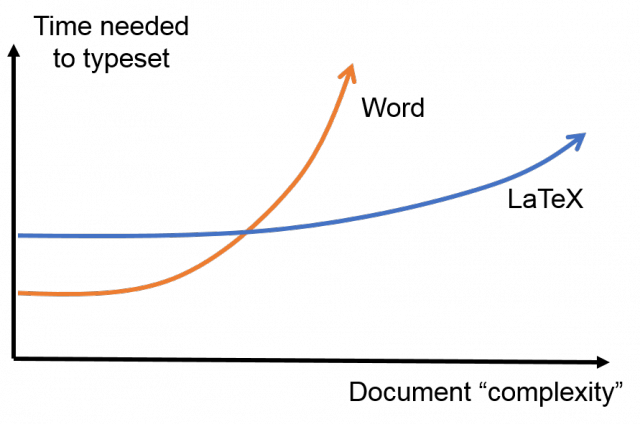
\includegraphics[width=10cm]{myplot1}
  \caption{Time vs Complexity}
\end{figure}

\subsection{Estimation of the material detached from the catchment as landslides}

\begin{tabular}{ l | c | r }
  1 & 2 & 3 \\ \hline
  4 & 5 & 6 \\
  7 & 8 & 9 \\
\end{tabular}


\begin{tabular}{ l | c | r }
\hline
  left & 2 & 3 \\ \hline
  left & center & right \\
  7 & 8 & 9 \\
\hline
\end{tabular}

\begin{table}[]
\centering

\label{my-label}
\begin{tabular}{lllll}
category & 1 & 2 & 3 & 4 \\ \hline
a        &   &   &   &   \\
b        &   &   &   &   \\
c        &   &   &   &  
\end{tabular}
\caption{My caption}
\end{table}

\begin{table}[]
\centering
\caption{My caption}
\label{my-label}
\begin{tabular}{lllll}
\hline
cat & A   & B   & C   & D   \\ \hline
1   & 0.5 & 0.5 & 0.5 & 0.5 \\
2   & 0.5 & 0.5 & 0.5 & 0.5 \\
3   & 0.5 & 0.5 & 0.5 & 0.5 \\ \hline
\end{tabular}
\end{table}

\begin{equation}
\sum x \frac{1}{2} \begin{bmatrix}
1 & 2 & 3\\ 
a & b & c\\ 
 &  & 
\end{bmatrix}
\end{equation}



\subsection{Regional Land Characteristics}
\subsubsection{Slope angle}
\subsubsection{Curvature}

\section{Results and Discussion}

\section{Conclusion}

\bibliography{myrefs}
\end{document}